\documentclass[xcolor=svgnames]{beamer}
\usepackage[utf8]{inputenc}
\usepackage[english]{babel}
%\usepackage{amssymb,amsmath}
%\usepackage[latin1]{inputenc}
%\usepackage{amsmath}
%\newcommand\abs[1]{\left|#1\right|}
\usepackage{amsmath}
\newcommand\abs[1]{\left|#1\right|}
\usepackage{hepnicenames}
\usepackage{hepunits}
\usepackage{color}
\usepackage{feynmp}
\usepackage{pst-pdf}
\usepackage{hyperref}
\usepackage{xcolor}
\hypersetup{colorlinks=true}
\usepackage{booktabs}


\setbeamertemplate{footline}{\insertframenumber/\inserttotalframenumber}
%%%%%%%%%%%%%%%%%%%%%%%%%%%%%%%%%%%%%%%%%%%%%%%%%%%%%%%%%%%%%%%%%%5
\definecolor{mygreen}{cmyk}{0.82,0.11,1,0.25}



%\DeclareCaptionFont{uiblack}{\color{uiblack}}
%\DeclareCaptionFont{uipoppy}{\color{uipoppy}}
%\captionsetup{labelfont={uipoppy},textfont=uiblack}

% see the macros.tex file for definitions


\renewcommand{\PKs}{{\HepParticle{K}{S}{}\xspace}}
\newcommand{\at}{\makeatletter @\makeatother}
%\renewcommand{\inserttotalframenumber}{\pageref{lastslide}}
\newcommand{\beginbackup}{
   \newcounter{framenumbervorappendix}
   \setcounter{framenumbervorappendix}{\value{framenumber}}
}
\newcommand{\backupend}{
   \addtocounter{framenumbervorappendix}{-\value{framenumber}}
   \addtocounter{framenumber}{\value{framenumbervorappendix}} 
}

%--------------------------------------------------------------------
%                           Introduction
%--------------------------------------------------------------------

\usetheme{Sybila} 

\title{LHCb Topological Trigger Reoptimization}
\author{Philip Iten$^{1}$, Tatiana Likhomanenko$^{2,3}$, \\
Egor Khairullin$^{2}$, Andrey Ustyuzhanin$^{2,3}$, Mike Williams$^{1}$}
%\footnotesize{on behalf of the LHCb collaboration}}
\institute{$^1$~Massachusetts Institute of Technology,~US \\
$^2$~Yandex School of Data Analysis,~RU \\
$^3$~NRC "Kurchatov Institute",~RU}

\date{\today}
\begin{document}
% --------------------------- SLIDE --------------------------------------------
\frame[plain]{\titlepage}
\author{T. Likhomanenko tatiana.likhomanenko@cern.ch}
% ------------------------------------------------------------------------------
% --------------------------- SLIDE --------------------------------------------



\institute{~}

%--------------------------------------------------------------------
%                          OUTLINE
%--------------------------------------------------------------------




\section[Outline]{}

\begin{frame}\frametitle{What is Topological Trigger?}
\begin{columns}
\column{3in}
\begin{itemize}
	\item Generic trigger for decays of beauty and charm hadrons
	\item It designed to be inclusive trigger line to efficiently select any B decay with at least 2 charged daughters	
	\item Look for 2, 3, 4 track combinations in a wide mass range
	\item Designed to efficiently select decays with missing particles
	\item Use fast-track fit to improve signal efficiency and minbias rejection
\end{itemize}
\column{2in}
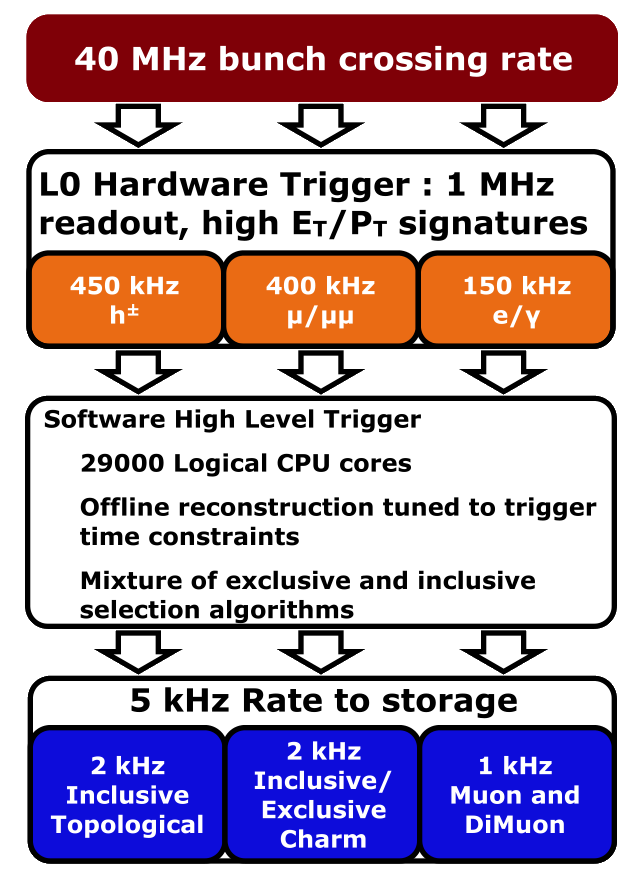
\includegraphics[width=1.9in]{images/triggers-system.png}

\end{columns}
\vspace*{0.3cm}
{\bf Goal:}  improve topological trigger efficiency for Run-2
\end{frame}


\begin{frame}\frametitle{Run-2 HLT Scheme}
\begin{columns}
\column{2in}
\hspace*{0.1cm} 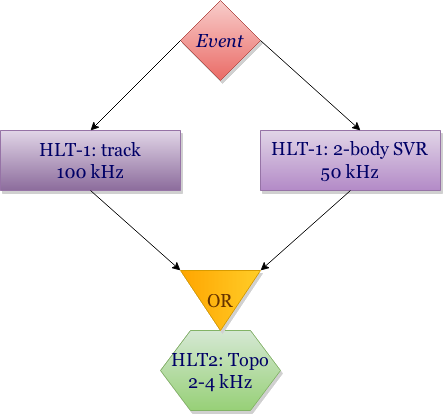
\includegraphics[width=1.9in]{images/sheme.png}
\column{2.8in}
What tells us an event contains interesting physics?

\begin{itemize}
\item A combination of displacement from PV and high PT
\end{itemize}

Run-2 strategy:
\begin{itemize}
\item HLT-1 track is looking for either one super high PT or high displacement track
\item HLT-1 2-body SVR classifier is looking for two tracks making a vertex 
\item HLT-2 improved topo classifier uses full reconstructed event to look for 2, 3, 4 and more tracks making a vertex

%	\item In Run 1 in HLT1 ("1 track") the track PT threshold was too high for an SVR-based approach to work
%	\item In Run 2 the HLT1 track PT threshold will be the same as HLT2 for Run 1 so~we~revisit "1 track" vs "2-body~SVR"
%	\item Consider HLT1 output rate (excluding special muon, electron lines) of 125 kHz to be split between "1 track" and "2-body~SVR" 
%	\item Consider Topo-trigger HLT2 output rate of 2-4 kHz
\end{itemize}

\end{columns}
\vspace*{0.5cm}

{\bf NOTE}: tracking thresholds are quite different in Run-1 and Run-2
\end{frame}


\begin{frame}\frametitle{N-body Tracks}
\begin{itemize}
\item Two, three or four tracks are combined to form a SVR
\item Each secondary vertex in Monte Carlo data is preselected in such way, that all tracks must be matched to particles from the signal decay (true match preselection)
\end{itemize}
\vspace*{1cm}

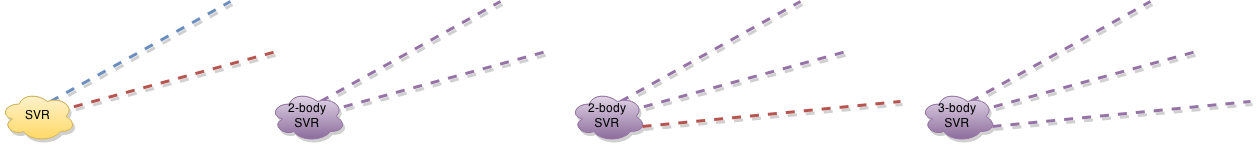
\includegraphics[width=4.5in, height=0.8in]{images/nbody.png}
\end{frame}

\begin{frame}\frametitle{Ommision of Daughters}
\hspace*{1.5cm}  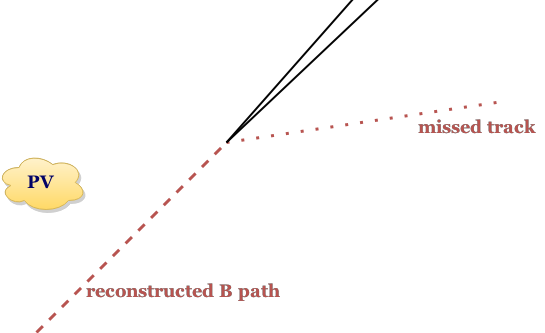
\includegraphics[width=3in]{images/ommited-2p.png}

\vspace*{0.5cm}

The trigger is designed to allow for the omission of one or more daughters when forming the trigger candidate.
\end{frame}

\begin{frame}\frametitle{Ommision of Daughters}
\hspace*{1cm}  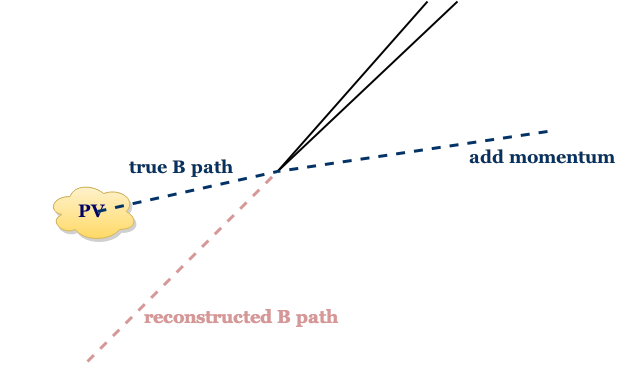
\includegraphics[width=3.5in]{images/ommited-2.png}

$$m_{corrected} = \sqrt{m^2 + \left | p_{Tmissing}^{'}\right |^2} + \left | p_{Tmissing}^{'} \right | $$
\end{frame}

\begin{frame}\frametitle{Machine Learning Specific Problem: data structure}
\begin{columns}
\column{3in}
\begin{itemize}
	\item Signal samples are simulated 13-TeV B decays of various topologies
	\item Background sample is generic Pythia 13-TeV proton-proton collisions
	\item Most events have many secondary vertices SVRs (not all events have an SVR)
\end{itemize}
\column{2in}
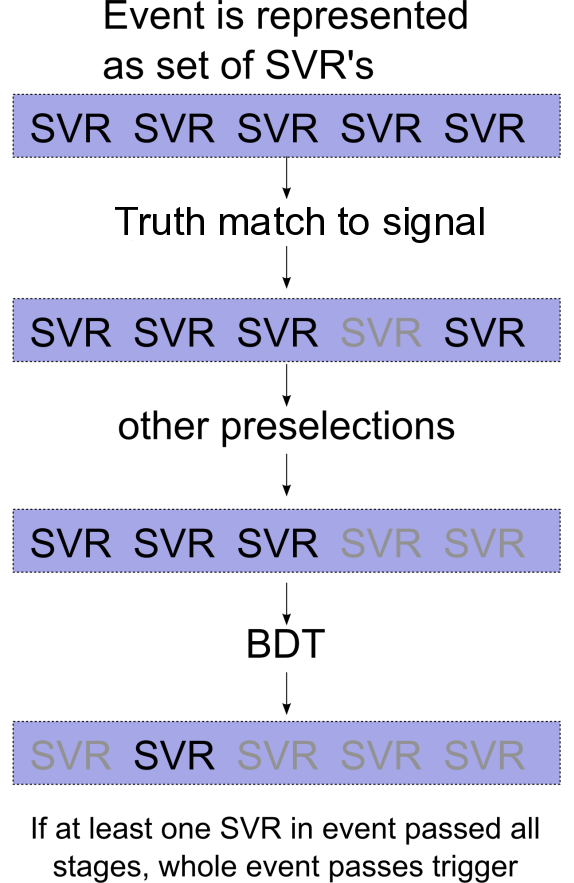
\includegraphics[width=1.9in]{images/triggers-svg.png}
\end{columns}
\end{frame}



\begin{frame}\frametitle{Machine Learning Specific Problem: FOM}
\begin{columns}
\column{3in}
\hspace*{0.2cm}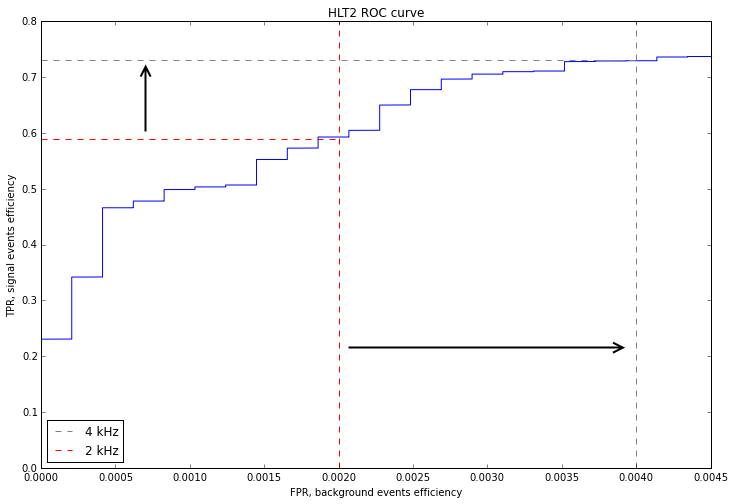
\includegraphics[width=2.8in]{images/roc_events.png}
\column{2in}
\begin{itemize}
	\item FOM is the over all efficiency, calculated for passed events, not SVRs
	\item Output rate must be limited
	\item Restriction is imposed on background events efficiency FPR = 0,2\% (corresponds to 2 kHz)
\end{itemize}
\end{columns}
\end{frame}




\begin{frame}\frametitle{HLT2: threshold unstability}
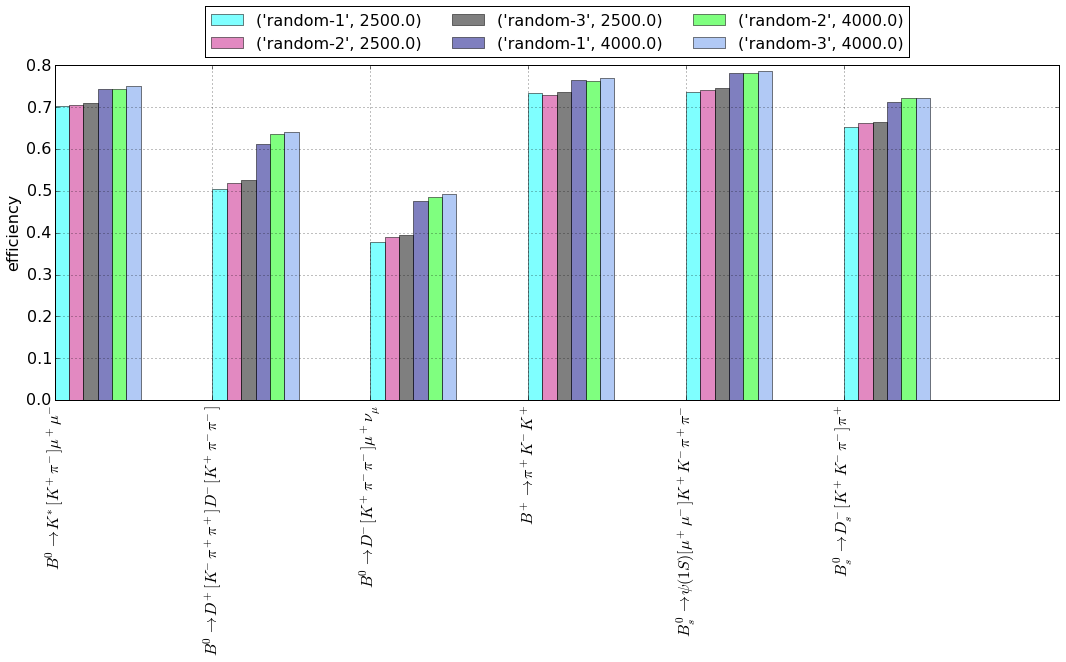
\includegraphics[width=4.5in]{images/random.png}
\end{frame}

\begin{frame}\frametitle{HLT2: efficiency vs output rate}
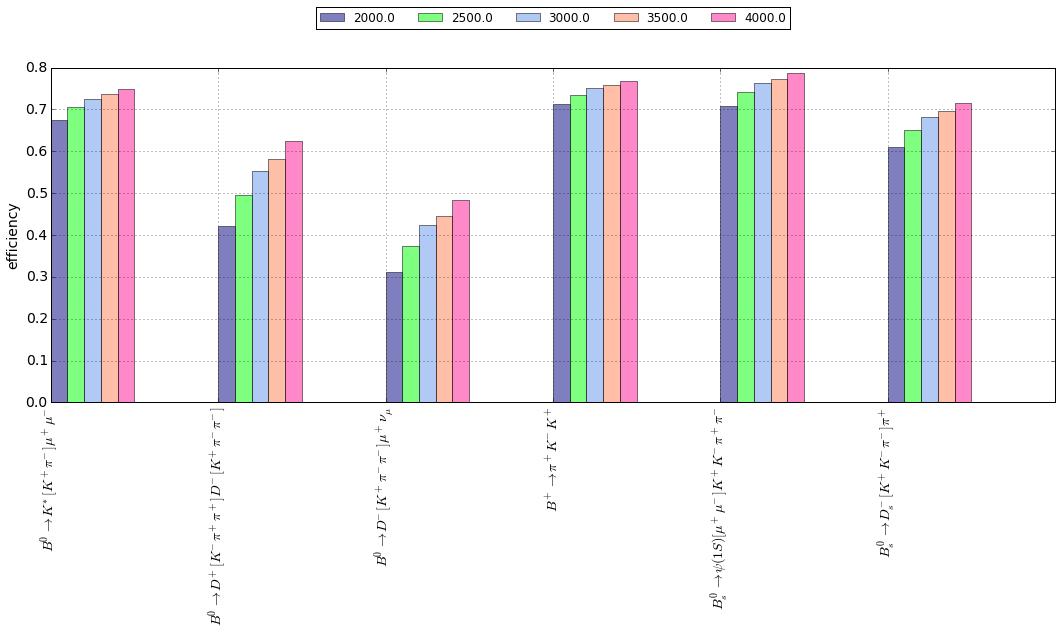
\includegraphics[width=4.5in]{images/rates_small.png}
\end{frame}




\begin{frame}\frametitle{Online Processing: BBDT vs Post-prunning}
\begin{columns}[T]
\column{2.4in}
\hspace*{1cm} {\bf Bonsai BDT (BBDT):}
\begin{itemize}
	\item Used in Run-1 for online processing
	\item Features hashing before training by yourself
	\item Convert decision trees to n-dimentional table making it essentially infinitely fast
	\item Predict operation takes one reading from this table
\end{itemize}
{\bf But: }
\begin{itemize}
	\item We are limited in the table size (or count of bins for each feature)
	\item Discretization reduces efficiency
\end{itemize}
\column{2.4in}
\hspace*{1cm} {\bf MatrixNet (MN) post-prunning:}
\begin{itemize}
	\item Another strategy for online processing
	\item Features also hashing with amount count of bins for each variable
	\item Post-prunning of the decision trees to speedup prediction operation (less count of trees)
	\item Online predict event by all trees
\end{itemize}
\end{columns}
\end{frame}


\begin{frame}\frametitle{BBDT vs Post-prunning Efficiencies}
\begin{center}
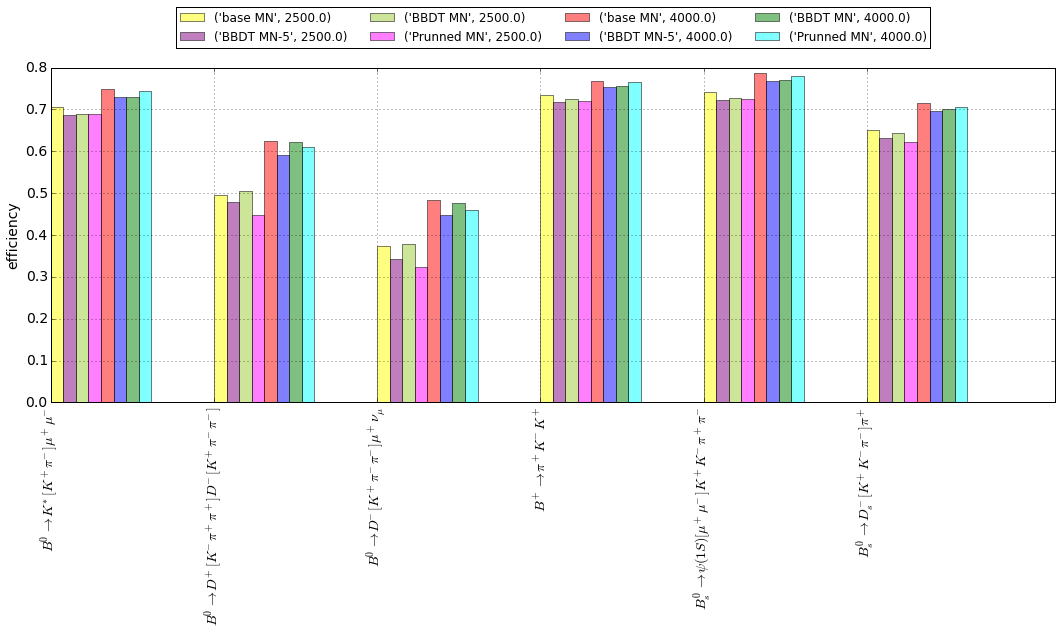
\includegraphics[width=4.5in]{images/prun-base.png} 
\end{center}
\end{frame}


\begin{frame}\frametitle{BBDT vs Post-prunning Efficiencies: ROCs}
\begin{center}
 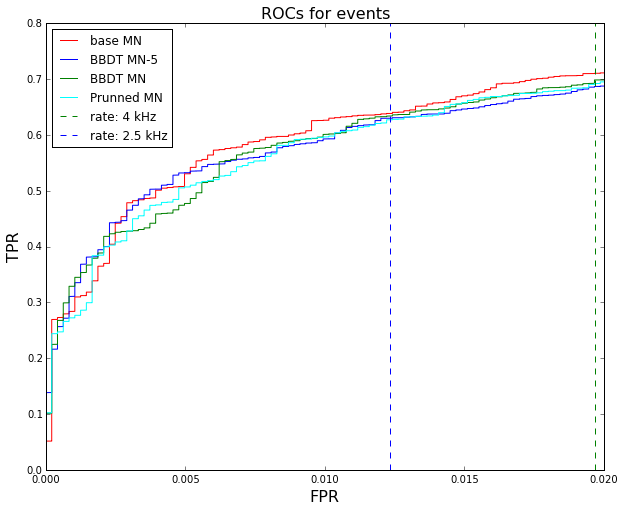
\includegraphics[width=3.5in]{images/prun-roc.png} 
 \end{center}
\end{frame}




\begin{frame}\frametitle{Current Status: Run-1 vs Run-2}
  \begin{center}
  Ratio of Run-2 over Run-1 for HLT2/HLT1 efficiencies
  \vspace{0.4cm}
  
    \begin{tabular}{c|c|c}
    mode & 2.5 kHz & 4. kHz  \\ \hline 
    $B^0\to K^*[K^+\pi^-]\mu^+\mu^-$ & 1.64 & 1.72   \\ 
    $B^+\to \pi^+K^-K^+$ & 1.59 & 1.65 \\ 
    $B^0_s\to D_s^-[K^+K^-\pi^-]\mu^+\nu_\mu$ & 1.14 & 1.47 \\ 
    $B^0_s\to \psi(1S)[\mu^+\mu^-]K^+K^-\pi^+\pi^-$ & 1.62 & 1.71 \\ 
    $B^0_s\to D_s^-[K^+K^-\pi^-]\pi^+$ & 1.46 & 1.52 \\ 
    $B^0\to D^+[K^-\pi^+\pi^+]D^-[K^+\pi^-\pi^-]$ & 1.40 & 1.86  \\ \hline

    \end{tabular}
\end{center}

%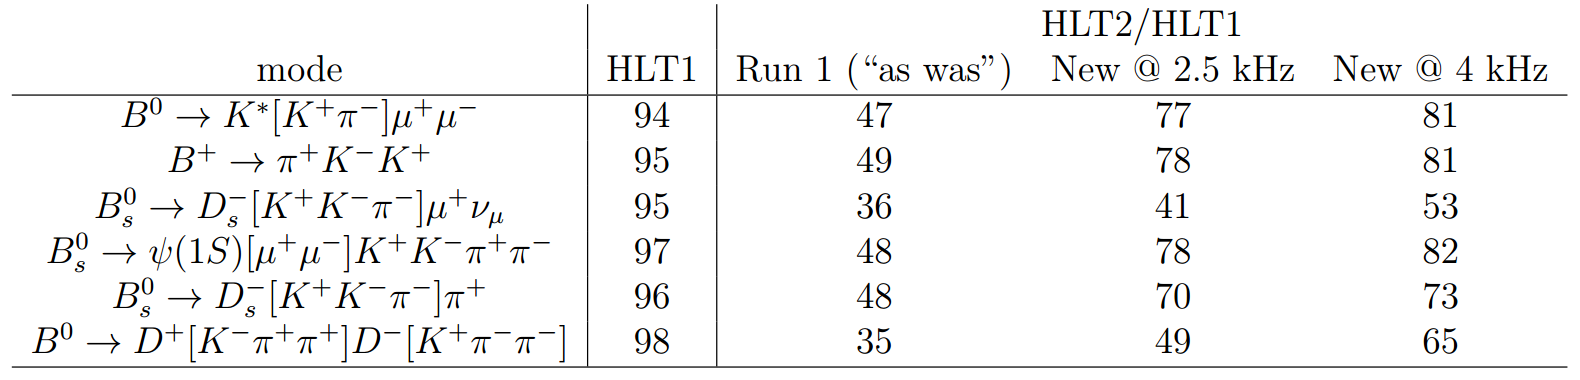
\includegraphics[width=4.5in]{images/run1run2.png}

\vspace{0.6cm}
Note that the denominator is reconstructible with $PT(B)>2$~GeV, $\tau(B)>0.2$~ps.
\end{frame}



\begin{frame}\frametitle{Summary}
\linespread{1.5}
\begin{enumerate}
\item New HLT scheme in Run-2: sophisticated HLT1 (classifier) and HLT2-Topo 
\item Overall (HLT2/HLT1) efficiency improvement: 15-60\% for 2.5~kHz (50-80\% for 4~kHz) vs Run-1
\item Timing comparison of MatrixNet BBDT vs post-pruning is in progress 
\item Looking forward to data taking!
\end{enumerate}

\end{frame}

\begin{frame}\frametitle{}
{
\begin{center} 
	\huge Thank you for attention!
\end{center}
}
\end{frame}

\beginbackup
\begin{frame}\frametitle{}  
\begin{center} 
	\huge Backup
\end{center}
\end{frame}

\begin{frame}\frametitle{HLT1-track and HLT1 2-body SVR preselections} 
\begin{columns}[T]
\column{1.7in}
\hspace*{1cm} {\bf 1 track:}
\begin{itemize}
	\item Tracks preselections: 
	      \begin{itemize}
	         \item $PT > 500$ MeV; 
	         \item $IP_{\chi^2} > 4$;
	         \item ${track}_{\chi^2} / ndof < 3;$
	       \end{itemize}
	\item BDT uses $PT$, $IP_{\chi^2}$
	\item Output rate 100 kHz
\end{itemize}
\column{3.2in}
\hspace*{1cm} {\bf 2-body SVR:}
\begin{itemize}
	\item Tracks preselections: 
     	       \begin{itemize}
	         \item $PT > 500$ MeV; 
	         \item $IP_{\chi^2} > 4$;
	         \item $track_{\chi^2}/ndof < 2.5;$
	       \end{itemize}
	\item SVR preselections:
   	      \begin{itemize}
	         \item $PT > 2$ GeV;
	         \item  $vertex_{\chi^2} < 10$;
		\item  $1 < MCOR$ GeV; 
		\item $2 < \eta < 5$ (PV to SVR)
	       \end{itemize}
	\item Don't use MCOR in BDT (from a systematics perspective)
	\item BDT variables: sum $PT$, $vertex_{\chi^2}$, $FD_{\chi^2}$,  $N$(tracks with $IP_{\chi^2}<16$~)
	\item Output rate 50 kHz
\end{itemize}
\end{columns}

\end{frame}

\begin{frame}\frametitle{HLT1-track: decision boundary}
\begin{columns}
  \column{2.5in}
	\hspace*{0.5cm} 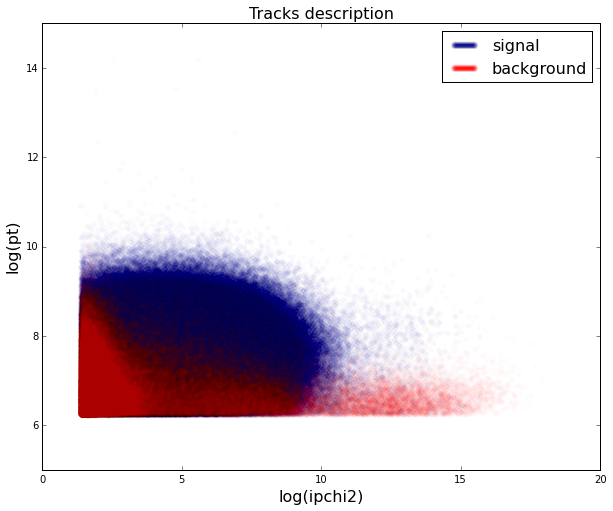
\includegraphics[width=1.9in]{images/track-db.png} \hfill
	\hspace*{0.5cm} 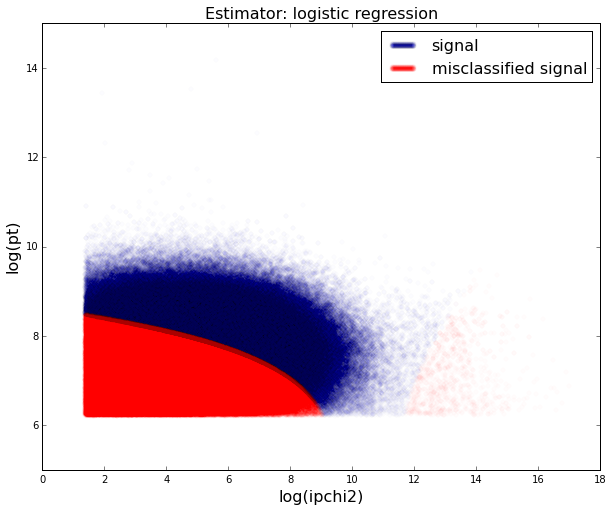
\includegraphics[width=1.9in]{images/log-track-db.png} \hfill
  \column{2.5in}
	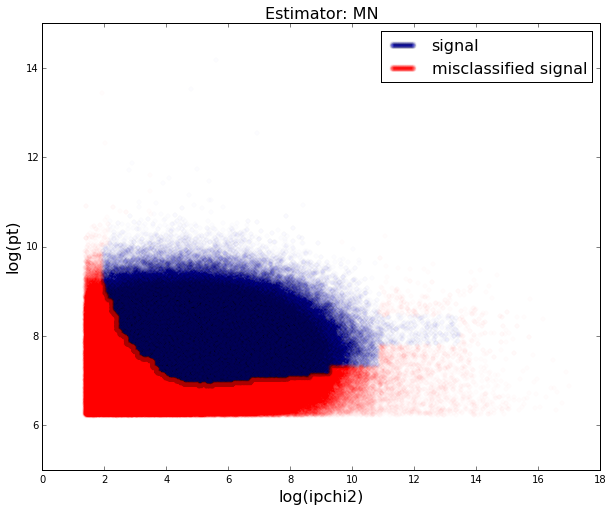
\includegraphics[width=1.9in]{images/mn-track-db.png} \hfill
	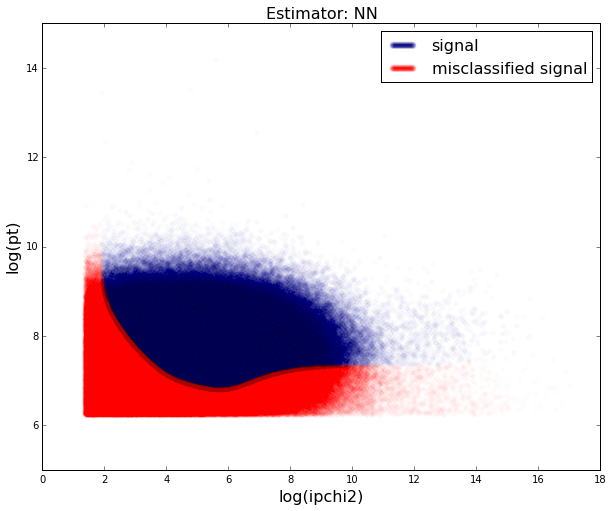
\includegraphics[width=1.9in]{images/nn-track-db.png} \hfill
\end{columns}
\end{frame}


\begin{frame}\frametitle{HLT1-track: MN vs NN vs logistic}
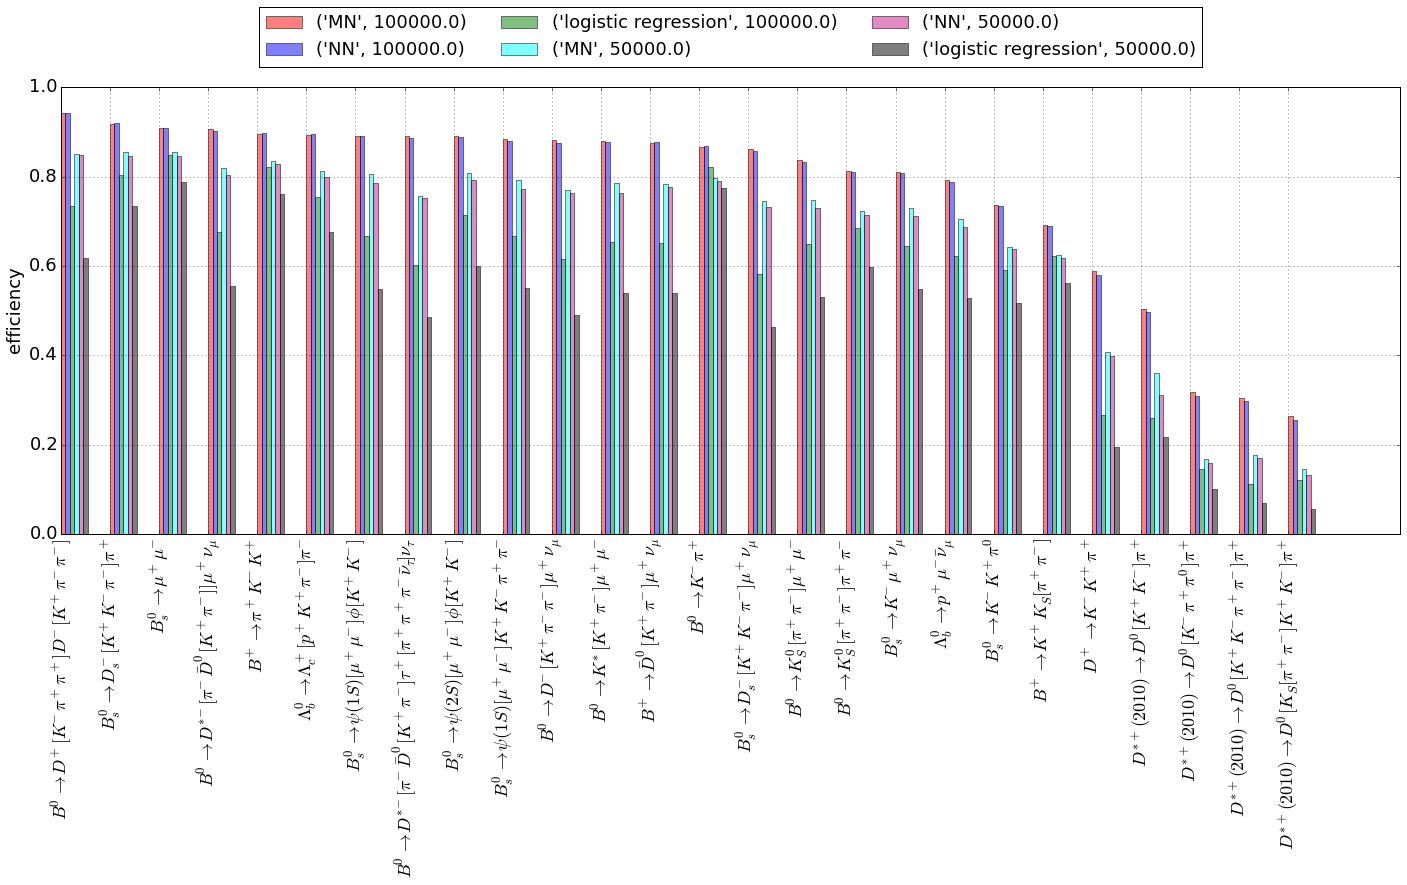
\includegraphics[width=4.5in]{images/track.png}
\end{frame}



\begin{frame}\frametitle{HLT1-SV}
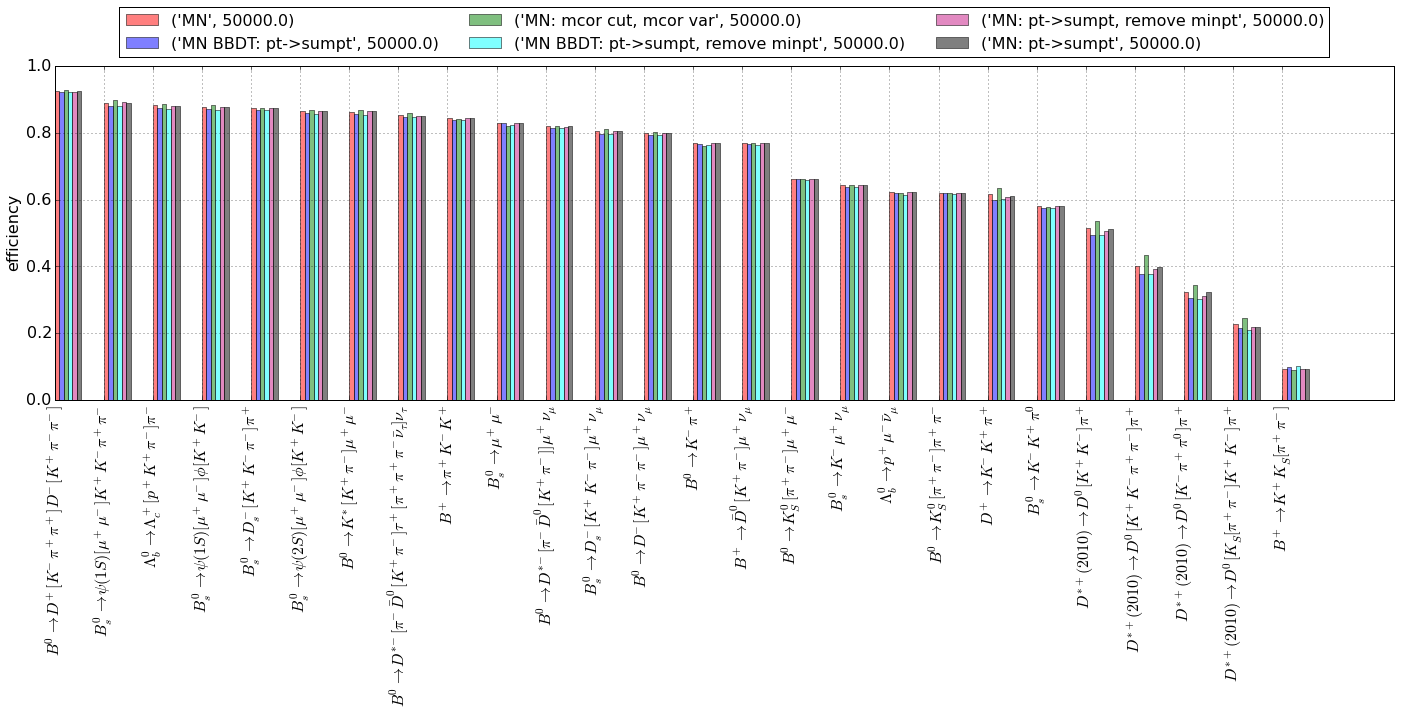
\includegraphics[width=4.5in]{images/hlt1-2body.png}
\end{frame}

\begin{frame}\frametitle{HLT2 preselections}
%\begin{columns}
%\column{1.5in}
\small{
\begin{itemize}
	\item The same preselections as for 2-body SVR 
	\item Changed track $PT > 200$~MeV
	\item Added $MCOR < 10$~GeV
	\item Added $N$(tracks with $IP_{\chi^2}<16) < 2$
	\item Used any min $PT$
	\item BDT variables: $n$, $MCOR$, sum $PT$, $vertex_{\chi^2}$, $\eta$, $FD_{\chi^2}$, min $PT$, $IP_{\chi^2}$,  $N$(tracks with $IP_{\chi^2}<16$~), $N(tracks)$
	\item Output rate 2-4 kHz
\end{itemize}
}
%\end{columns}

\end{frame}

\begin{frame}\frametitle{HLT2: n-bodies comparison}
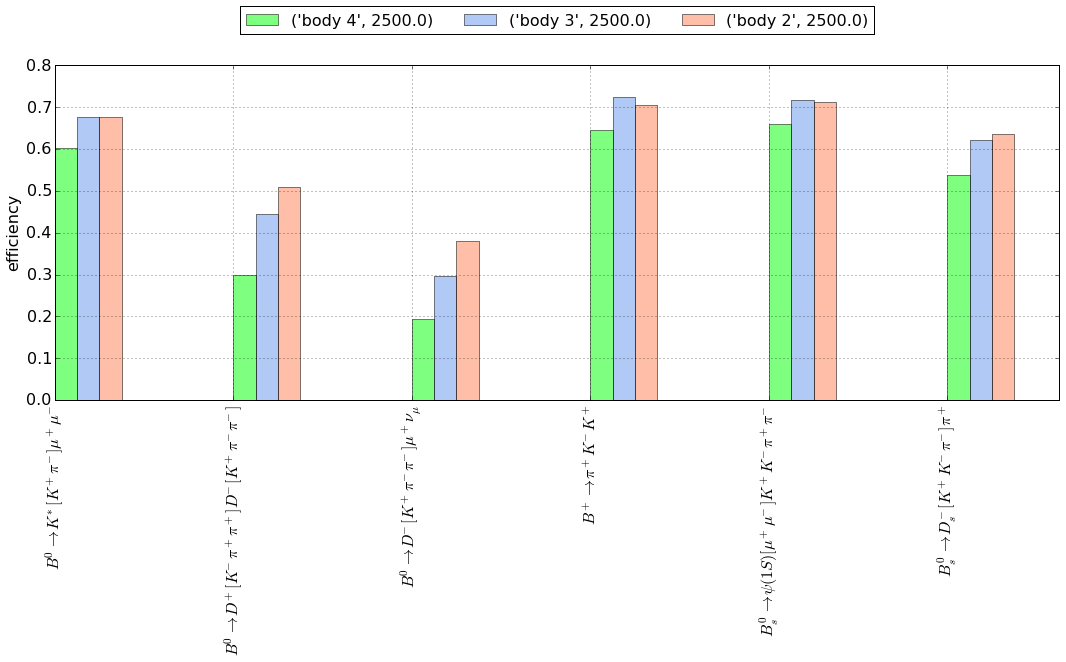
\includegraphics[width=4.5in]{images/bodies.png}
\end{frame}

\begin{frame}\frametitle{HLT2: n-bodies comparison for other modes}
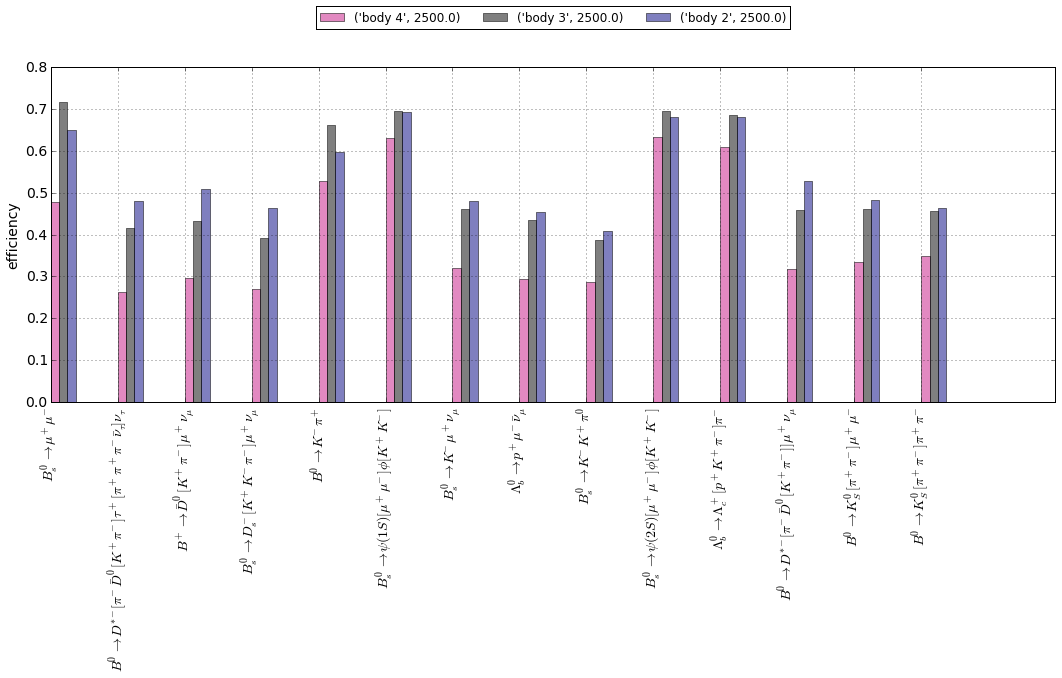
\includegraphics[width=4.5in]{images/hlt_body.png}
\end{frame}

\begin{frame}\frametitle{HLT2: models comparison}
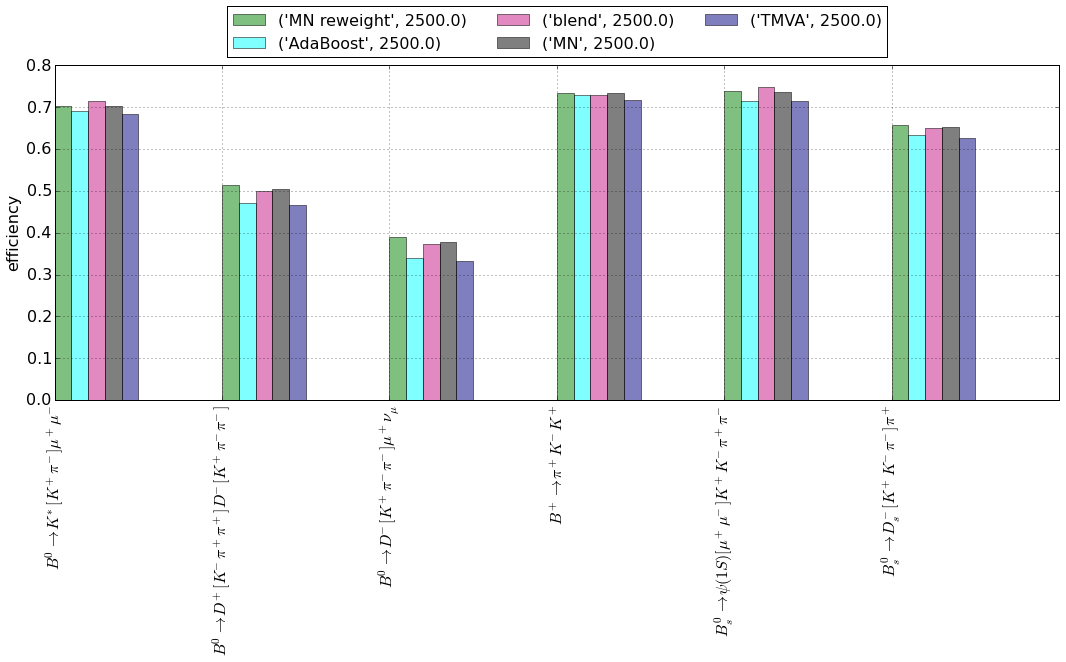
\includegraphics[width=4.5in]{images/blend.png}
\end{frame}

\begin{frame}\frametitle{HLT2: models comparison for other modes}
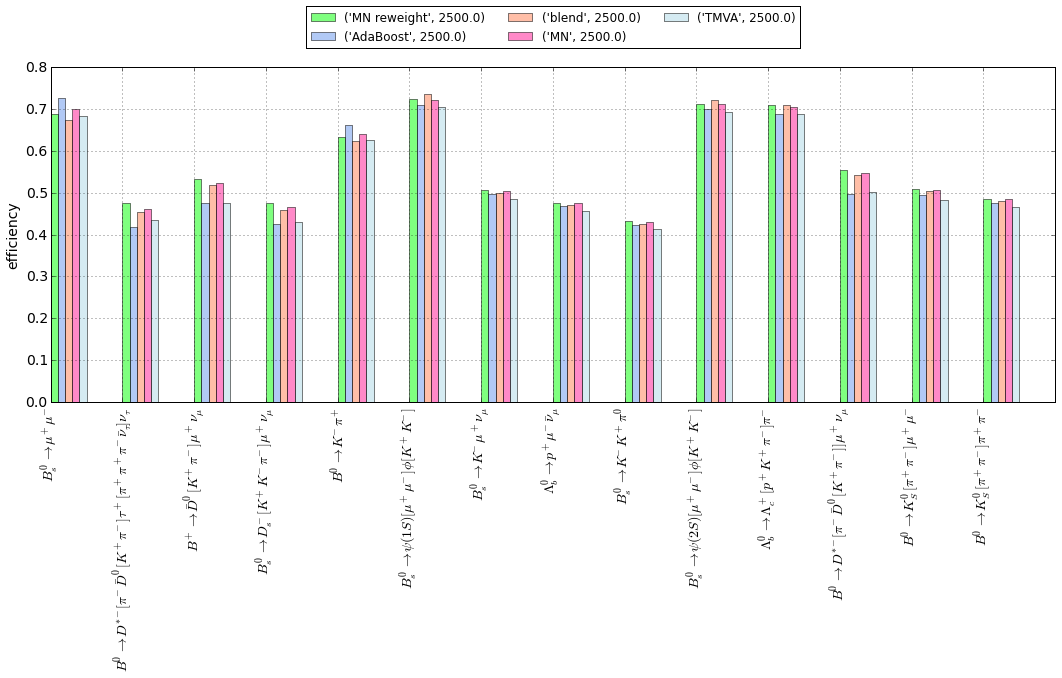
\includegraphics[width=4.5in]{images/hlt_mns.png}
\end{frame}

\begin{frame}\frametitle{HLT2: efficiency vs output rate for other modes}
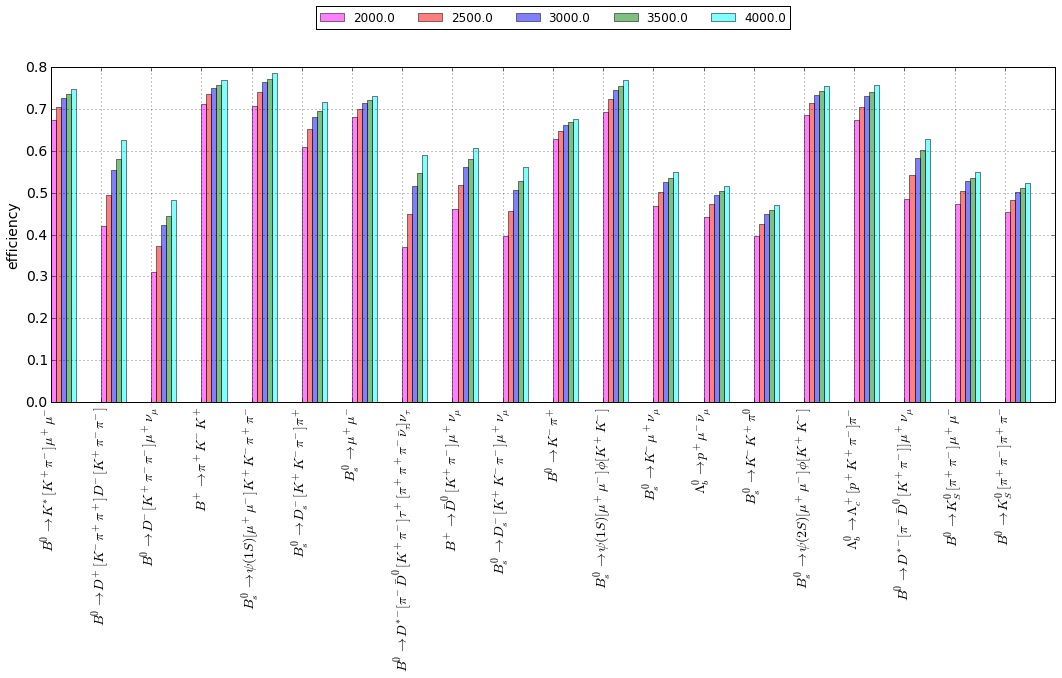
\includegraphics[width=4.5in]{images/rates.png}
\end{frame}

\begin{frame}\frametitle{BBDT vs Post-prunning efficiencies for other modes}
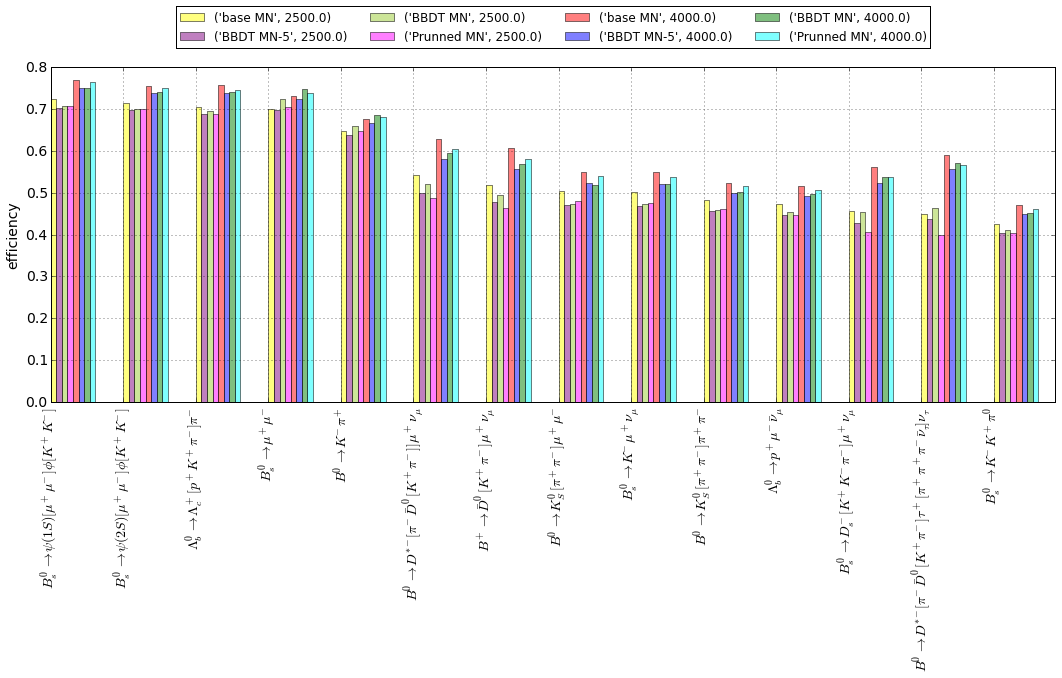
\includegraphics[width=4.5in]{images/prun.png}
\end{frame}
\backupend

\end{document}
